\chapter{Desenvolvimento do Sistema}\label{cap:dev_sist}

\section{O sistema}

O sistema dispõe de uma funcionalidade que auxilia as coordenadorias e departamentos nas definição dos encargos semestrais. Para isso, os cursos devem ser cadastrados ao sistema e administradores vinculados aos mesmos. A partir disso, eles passarão a ser responsáveis pelo seu gerenciamento. Professores poderão ser cadastrados para que possam se dispor a ministrar disciplinas, informando dados sobre a mesma e sobre sua própria disponibilidade de horário. Por fim, o sistema auxiliará a administração das Coordenadorias nas definições de disciplinas e seus professores, avaliação dos planos de ensino, e por último, definir o quadro de horário do devido semestre.

\section{Requisitos}\label{section:dev:req}

\subsection{Atores}
O sistema dispõem de diferentes tipos de usuários que desempenham seus devidos papeis, sendo estes:

    \begin{description}
        \item[Administrador Geral:] Responsável pelo gerenciamento geral do sistema. É encarregado de criar os cursos e atribuir administradores aos mesmos. 
        \item[Administrador de Curso:] Qualificação usualmente atribuída aos Coordenadores, Vice Coordenadores e Secretários dos cursos, são responsáveis pelo gerenciamento específicos do seu curso, como informações básicas do mesmo, gestão dos usuários Professores, Membros do Colegiado e definição de horários.
        \item[Professor:] Papel atribuído aos professores dos cursos. Dentre outras responsabilidades, esses deverão se dispor a ministrar disciplinas, apresentando informações sobre as mesmas, como numero de vagas, plano de ensino e necessidade de laboratórios.
        \item[Membro do colegiado:] Usuários que serão responsáveis pela avaliação dos planos de ensino das disciplinas.
        \item[Chefe de Departamento:] Usuários que serão responsáveis pela gerenciamento dos Departamentos.
    \end{description}

\newpage
\subsection{Casos de uso}\label{subsec:casosdeuso}

lorem


\begin{figure}[h]
    \centering
    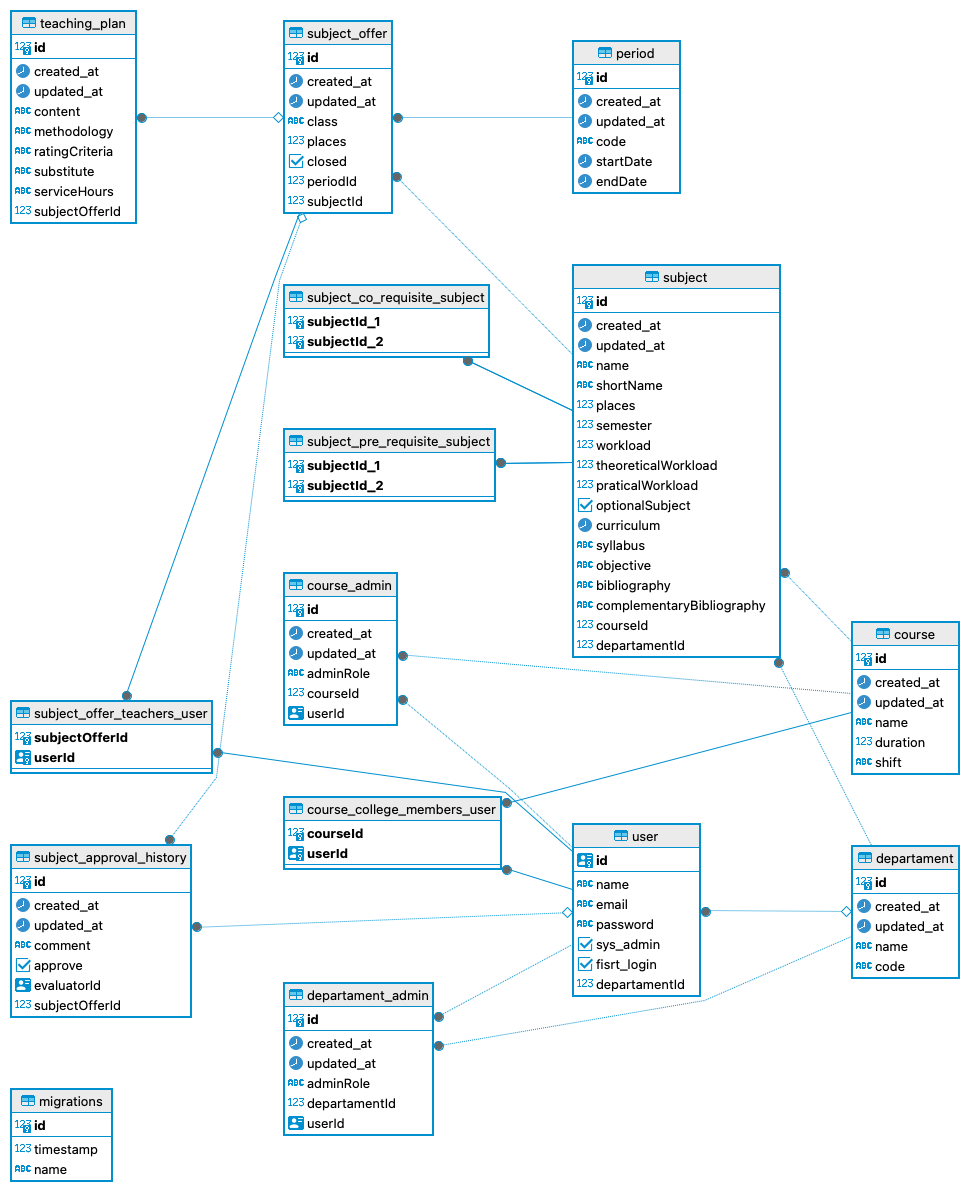
\includegraphics[width=450px]{imgs/model_db.png}
    \caption{Diagrama Casos de Uso.}
    \label{fig:Figura1}
\end{figure}